\chapter{Đặt vấn đề và phân tích dữ liệu}

\section{Bối cảnh và mục tiêu}
Bỏ học giữa chừng là một vấn đề mà các cơ sở giáo dục cần quan tâm. Khi sinh viên gặp khó khăn về học tập, tài chính hoặc hoàn cảnh cá nhân, việc nhà trường biết sớm có thể giúp việc tư vấn được thực hiện kịp thời hơn. Tuy nhiên, những nguyên nhân này không phải lúc nào cũng thể hiện rõ trong hồ sơ nhập học. Vì vậy, dự đoán bằng học máy chỉ có thể cung cấp thêm một căn cứ để xem xét, chứ không thể thay thế trao đổi trực tiếp với sinh viên.

Kết quả của dự án hướng đến hai nhóm đối tượng chính: (1) \textbf{cố vấn học tập và bộ phận hỗ trợ sinh viên} dùng danh sách cảnh báo để ưu tiên tiếp cận sớm; (2) \textbf{ban quản lý đào tạo} dùng phân tích lỗi theo ngành và nhóm tuổi để thiết kế chính sách hỗ trợ có mục tiêu. Mô hình được thiết kế như một công cụ sàng lọc bổ trợ, không thay thế phán xét của con người.

Trong bài tập này, nhóm sử dụng bộ dữ liệu \textit{Predict Students' Dropout and Academic Success} do UCI công bố \cite{uci}. Mục tiêu là xây dựng chương trình dự đoán trạng thái của một sinh viên khi đến cuối thời hạn chuẩn của khóa học. Dự đoán được đặt tại thời điểm nhập học, nghĩa là mô hình chỉ nên nhận những thông tin có thể biết vào thời điểm đó. Bộ dữ liệu có ba nhãn:
\begin{itemize}
    \item \textbf{Dropout}: sinh viên đã bỏ học.
    \item \textbf{Enrolled}: sinh viên vẫn đang theo học tại thời điểm ghi nhận kết quả.
    \item \textbf{Graduate}: sinh viên đã tốt nghiệp.
\end{itemize}
Nhóm giữ nguyên ba nhãn thay vì gộp Enrolled vào Dropout. Một sinh viên còn học sau thời hạn chuẩn không nhất thiết sẽ bỏ học; nếu gộp hai trạng thái, kết quả sẽ khó diễn giải hơn và làm thay đổi bài toán gốc.

Ngoài việc xây dựng mô hình, nhóm muốn trả lời hai câu hỏi: thay đổi cách biểu diễn đặc trưng có làm kết quả thay đổi không, và K-NN hay cây quyết định phân loại tốt hơn? Hai luồng dùng cùng 18 cột đầu vào, cùng cách chia và fold; luồng B tạo thêm hai đặc trưng từ các cột này.

\section{Nguồn và cấu trúc dữ liệu}
Bộ dữ liệu được công bố bởi Realinho và cộng sự trên UCI Machine Learning Repository, có mã DOI và được cấp phép CC BY 4.0 \cite{uci}. Dữ liệu được tổng hợp từ một cơ sở giáo dục đại học với nhiều ngành học. Mỗi dòng trong tệp tương ứng một sinh viên; các cột gồm thông tin nhân khẩu, quá trình đăng ký, kết quả học tập và trạng thái đầu ra.

Tệp \texttt{data.csv} của nhóm có 4.424 dòng và 37 cột, trong đó 36 cột là đặc trưng và cột \texttt{Target} là nhãn. Tệp sử dụng dấu chấm phẩy để phân cách các cột. Một điểm cần chú ý khi đọc dữ liệu là tên cột \texttt{Daytime/evening attendance} trong CSV gốc có ký tự tab ở cuối. Chương trình loại khoảng trắng ở đầu và cuối tên cột trước khi kiểm tra cấu trúc; nếu tập cột hoặc tập nhãn khác dự kiến, chương trình dừng và báo lỗi.

Theo UCI, bộ dữ liệu đã được xử lý các giá trị thiếu và bất thường trước khi công bố. Do đó, các nhận xét dưới đây chỉ phản ánh tệp đã tải, không phản ánh toàn bộ quá trình làm sạch dữ liệu ban đầu của tác giả. Trong lần kiểm tra của nhóm, tệp không có ô trống và không có dòng trùng hoàn toàn.

Bảng~\ref{tab:columns} tóm tắt ý nghĩa và loại sử dụng của 18 cột đầu vào; các biến phân loại được lưu dưới dạng số nguyên. Bảng tiếp theo liệt kê từng cột còn lại và kiểu lưu trong CSV.

\begin{table}[H]\centering\small
\caption{Ý nghĩa và kiểu dữ liệu các cột chính}\label{tab:columns}
\begin{tabular}{>{\raggedright\arraybackslash}p{5.2cm}>{\raggedright\arraybackslash}p{2cm}>{\raggedright\arraybackslash}p{5.8cm}}\toprule
Tên cột & Kiểu & Mô tả\\\midrule
Application order & Số nguyên & Thứ tự nguyện vọng (0 = ưu tiên nhất)\\
Previous qualification (grade) & Thực & Điểm văn bằng trước (thang 0–200)\\
Admission grade & Thực & Điểm tuyển sinh (thang 0–200)\\
Age at enrollment & Số nguyên & Tuổi lúc nhập học\\
Marital status & Phân loại & Tình trạng hôn nhân (mã số UCI)\\
Application mode & Phân loại & Hình thức đăng ký (mã số UCI)\\
Course & Phân loại & Mã ngành học\\
Daytime/evening attendance & Phân loại & Ca học (1 = ban ngày, 0 = tối)\\
Previous qualification & Phân loại & Loại bằng trước khi nhập học\\
Nacionality & Phân loại & Quốc tịch\\
Mother's qualification & Phân loại & Trình độ học vấn của mẹ\\
Father's qualification & Phân loại & Trình độ học vấn của cha\\
Mother's occupation & Phân loại & Nghề nghiệp của mẹ\\
Father's occupation & Phân loại & Nghề nghiệp của cha\\
Displaced & Phân loại & Chuyển nơi ở (1 = có, 0 = không)\\
Educational special needs & Phân loại & Nhu cầu giáo dục đặc biệt\\
Gender & Phân loại & Giới tính (1 = nam, 0 = nữ)\\
International & Phân loại & Sinh viên quốc tế (1 = có, 0 = không)\\\midrule
Target & Phân loại & Nhãn: Dropout / Enrolled / Graduate\\\bottomrule
\end{tabular}
\par\smallskip\small Phân loại là vai trò logic; trong CSV, các mã này là số nguyên. Target là chuỗi. Các cột còn lại được liệt kê ở bảng tiếp theo.\normalsize
\end{table}

\begin{longtable}{>{\raggedright\arraybackslash}p{6.3cm}p{1.5cm}>{\raggedright\arraybackslash}p{5.2cm}}
\caption{Ý nghĩa và kiểu dữ liệu 18 cột không dùng làm đầu vào}\\\toprule
Tên cột & Kiểu CSV & Ý nghĩa\\\midrule\endfirsthead
\toprule Tên cột & Kiểu CSV & Ý nghĩa\\\midrule\endhead
Debtor & int64 & Mã tình trạng nợ\\
Tuition fees up to date & int64 & Mã tình trạng học phí\\
Scholarship holder & int64 & Mã tình trạng học bổng\\
Curricular units 1st sem (credited) & int64 & Số học phần được công nhận, học kỳ 1\\
Curricular units 1st sem (enrolled) & int64 & Số học phần đã đăng ký, học kỳ 1\\
Curricular units 1st sem (evaluations) & int64 & Số lần đánh giá, học kỳ 1\\
Curricular units 1st sem (approved) & int64 & Số học phần đã hoàn thành, học kỳ 1\\
Curricular units 1st sem (grade) & float64 & Điểm học kỳ, học kỳ 1\\
Curricular units 1st sem (without evaluations) & int64 & Số học phần không có đánh giá, học kỳ 1\\
Curricular units 2nd sem (credited) & int64 & Số học phần được công nhận, học kỳ 2\\
Curricular units 2nd sem (enrolled) & int64 & Số học phần đã đăng ký, học kỳ 2\\
Curricular units 2nd sem (evaluations) & int64 & Số lần đánh giá, học kỳ 2\\
Curricular units 2nd sem (approved) & int64 & Số học phần đã hoàn thành, học kỳ 2\\
Curricular units 2nd sem (grade) & float64 & Điểm học kỳ, học kỳ 2\\
Curricular units 2nd sem (without evaluations) & int64 & Số học phần không có đánh giá, học kỳ 2\\
Unemployment rate & float64 & Tỷ lệ thất nghiệp\\
Inflation rate & float64 & Tỷ lệ lạm phát\\
GDP & float64 & Tổng sản phẩm quốc nội\\
\bottomrule\end{longtable}

\section{Phân bố nhãn}
Bảng \ref{tab:labels} trình bày số lượng của từng lớp trên toàn bộ dữ liệu và sau khi chia train/test. Nhóm chia phân tầng theo nhãn để tỷ lệ các lớp giữa hai tập không chênh lệch quá nhiều.
\begin{table}[H]\centering
\caption{Số lượng mẫu của từng lớp}\label{tab:labels}
\begin{tabular}{lrrrr}\toprule
Nhãn & Toàn bộ & Tỷ lệ toàn bộ & Train & Test\\\midrule
Dropout & 1.421 & 32,1\% & 1.137 & 284\\
Enrolled & 794 & 17,9\% & 635 & 159\\
Graduate & 2.209 & 49,9\% & 1.767 & 442\\\midrule
Tổng & 4.424 & 100\%* & 3.539 & 885\\\bottomrule
\end{tabular}
\par\smallskip\small * Các tỷ lệ được làm tròn riêng.\normalsize
\end{table}
Lớp Graduate chiếm gần một nửa dữ liệu, trong khi Enrolled chỉ chiếm khoảng 18\%. Sự mất cân bằng này ảnh hưởng đến cách đánh giá: một mô hình thiên về Graduate có thể đạt accuracy không thấp nhưng vẫn dự đoán kém hai lớp còn lại. Vì vậy, bên cạnh accuracy, nhóm theo dõi precision, recall và F1 cho từng lớp, đặc biệt là recall của Dropout.
\begin{figure}[H]\centering
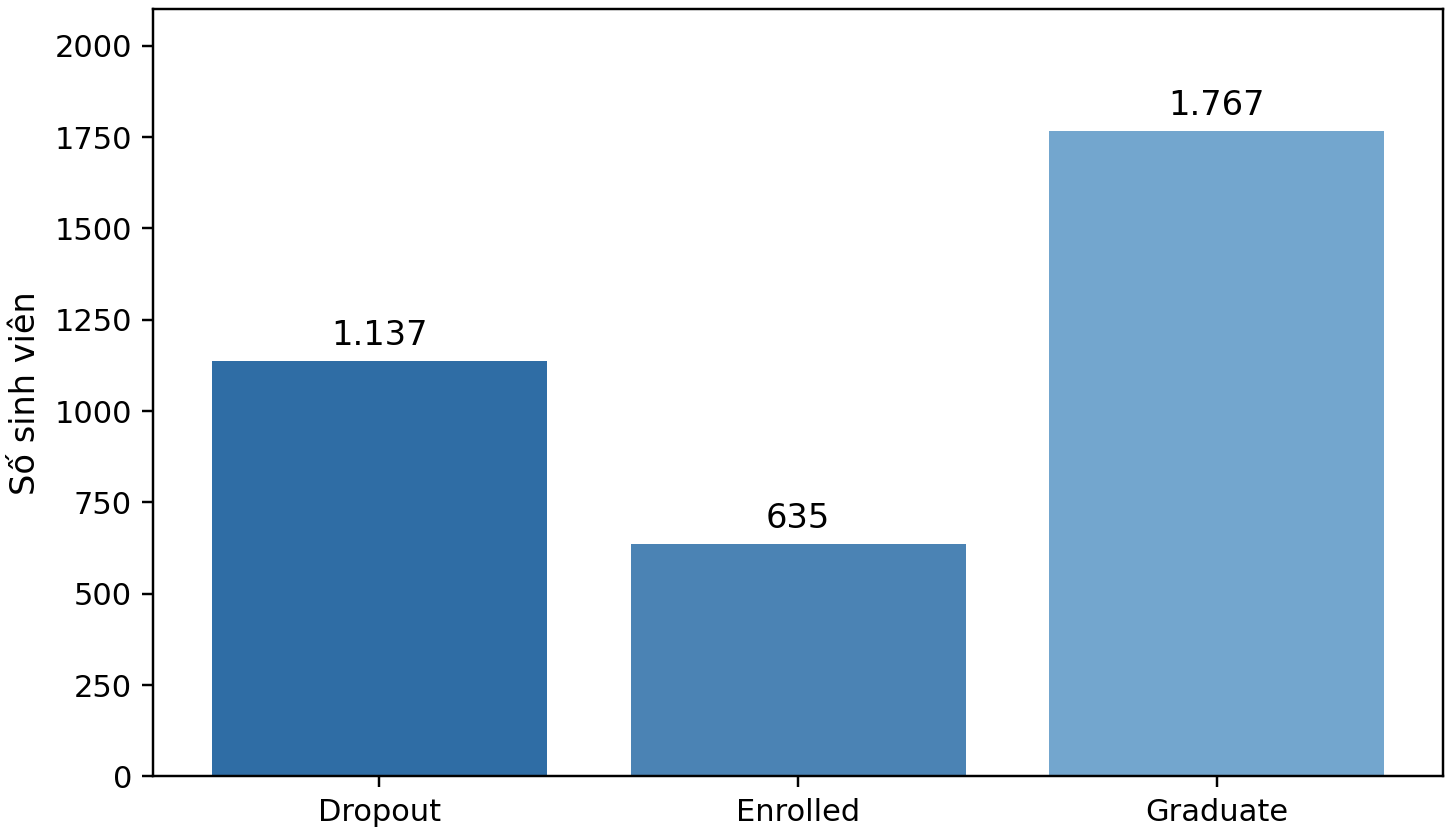
\includegraphics[width=.85\textwidth]{images/results/class_distribution.png}
\caption{Phân bố nhãn trên tập huấn luyện}\label{fig:classes}
\end{figure}

\section{Khám phá các đặc trưng}
\subsection{Biến số}
Với các biến số được sử dụng, nhóm xem giá trị nhỏ nhất, lớn nhất, trung vị, tứ phân vị và hình dạng phân phối trên tập train. Tuổi nhập học có trung vị 20, tứ phân vị thứ nhất là 19, tứ phân vị thứ ba là 25; giá trị nhỏ nhất và lớn nhất lần lượt là 17 và 70. Điều này cho thấy phần lớn sinh viên trong mẫu vào học ở độ tuổi tương đối trẻ, nhưng cũng có một nhóm nhập học ở độ tuổi lớn hơn.

Nhóm dùng quy tắc $1{,}5\times IQR$ để đánh dấu các giá trị nằm xa khoảng tứ phân vị. Trên tập train, số giá trị bị đánh dấu là 431 ở thứ tự nguyện vọng, 135 ở điểm văn bằng trước, 68 ở điểm tuyển sinh và 358 ở tuổi nhập học. Đây là dấu hiệu cần xem xét, không tự động là lỗi. Chẳng hạn, sinh viên lớn tuổi hơn vẫn là một trường hợp có thể xảy ra; vì vậy nhóm không xóa các dòng này.
\begin{figure}[H]\centering
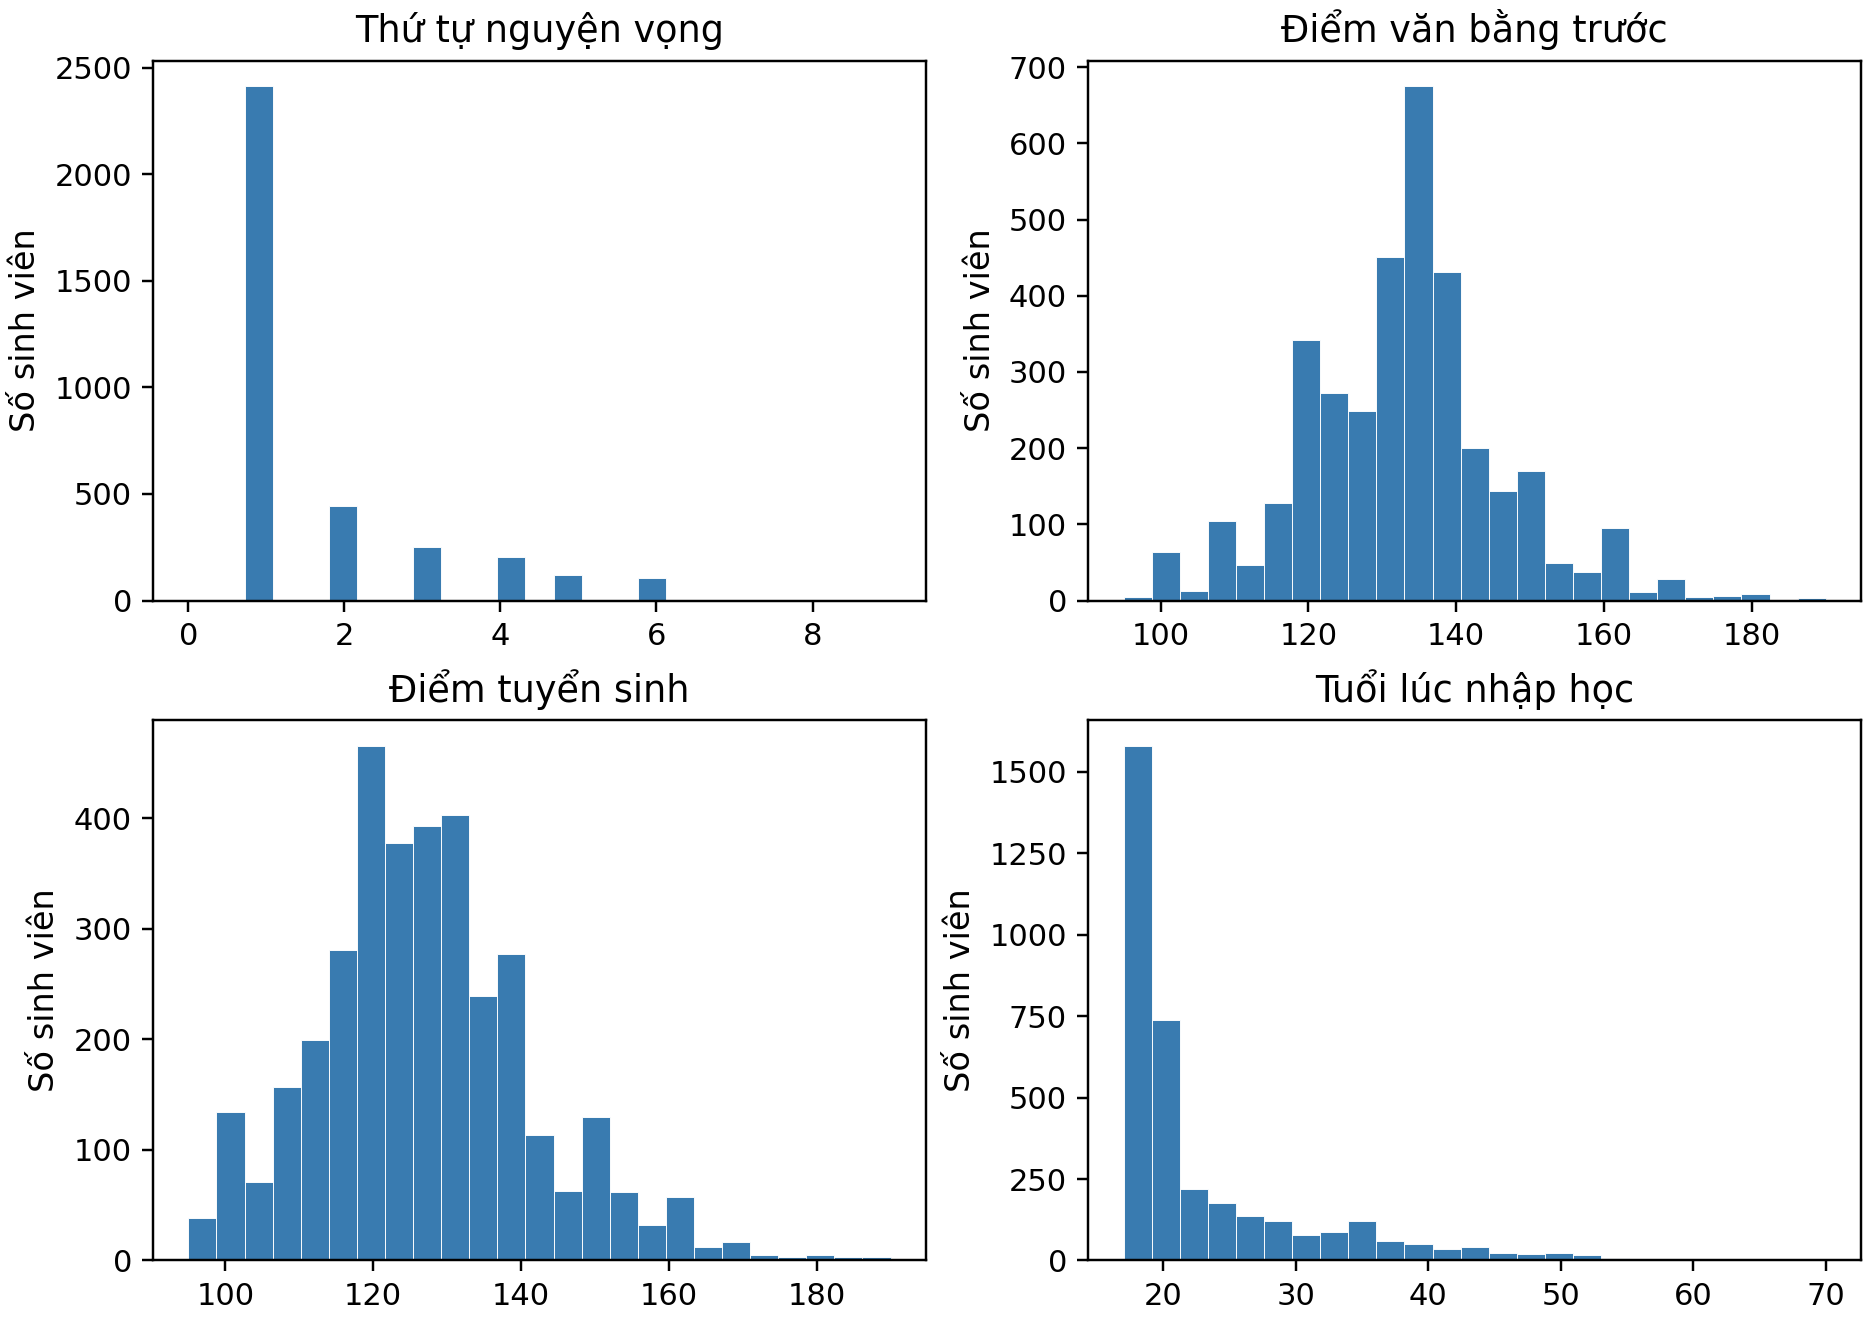
\includegraphics[width=.95\textwidth]{images/results/histograms.png}
\caption{Phân phối các biến số được chọn trên tập train}\label{fig:eda}
\end{figure}
\begin{figure}[H]\centering
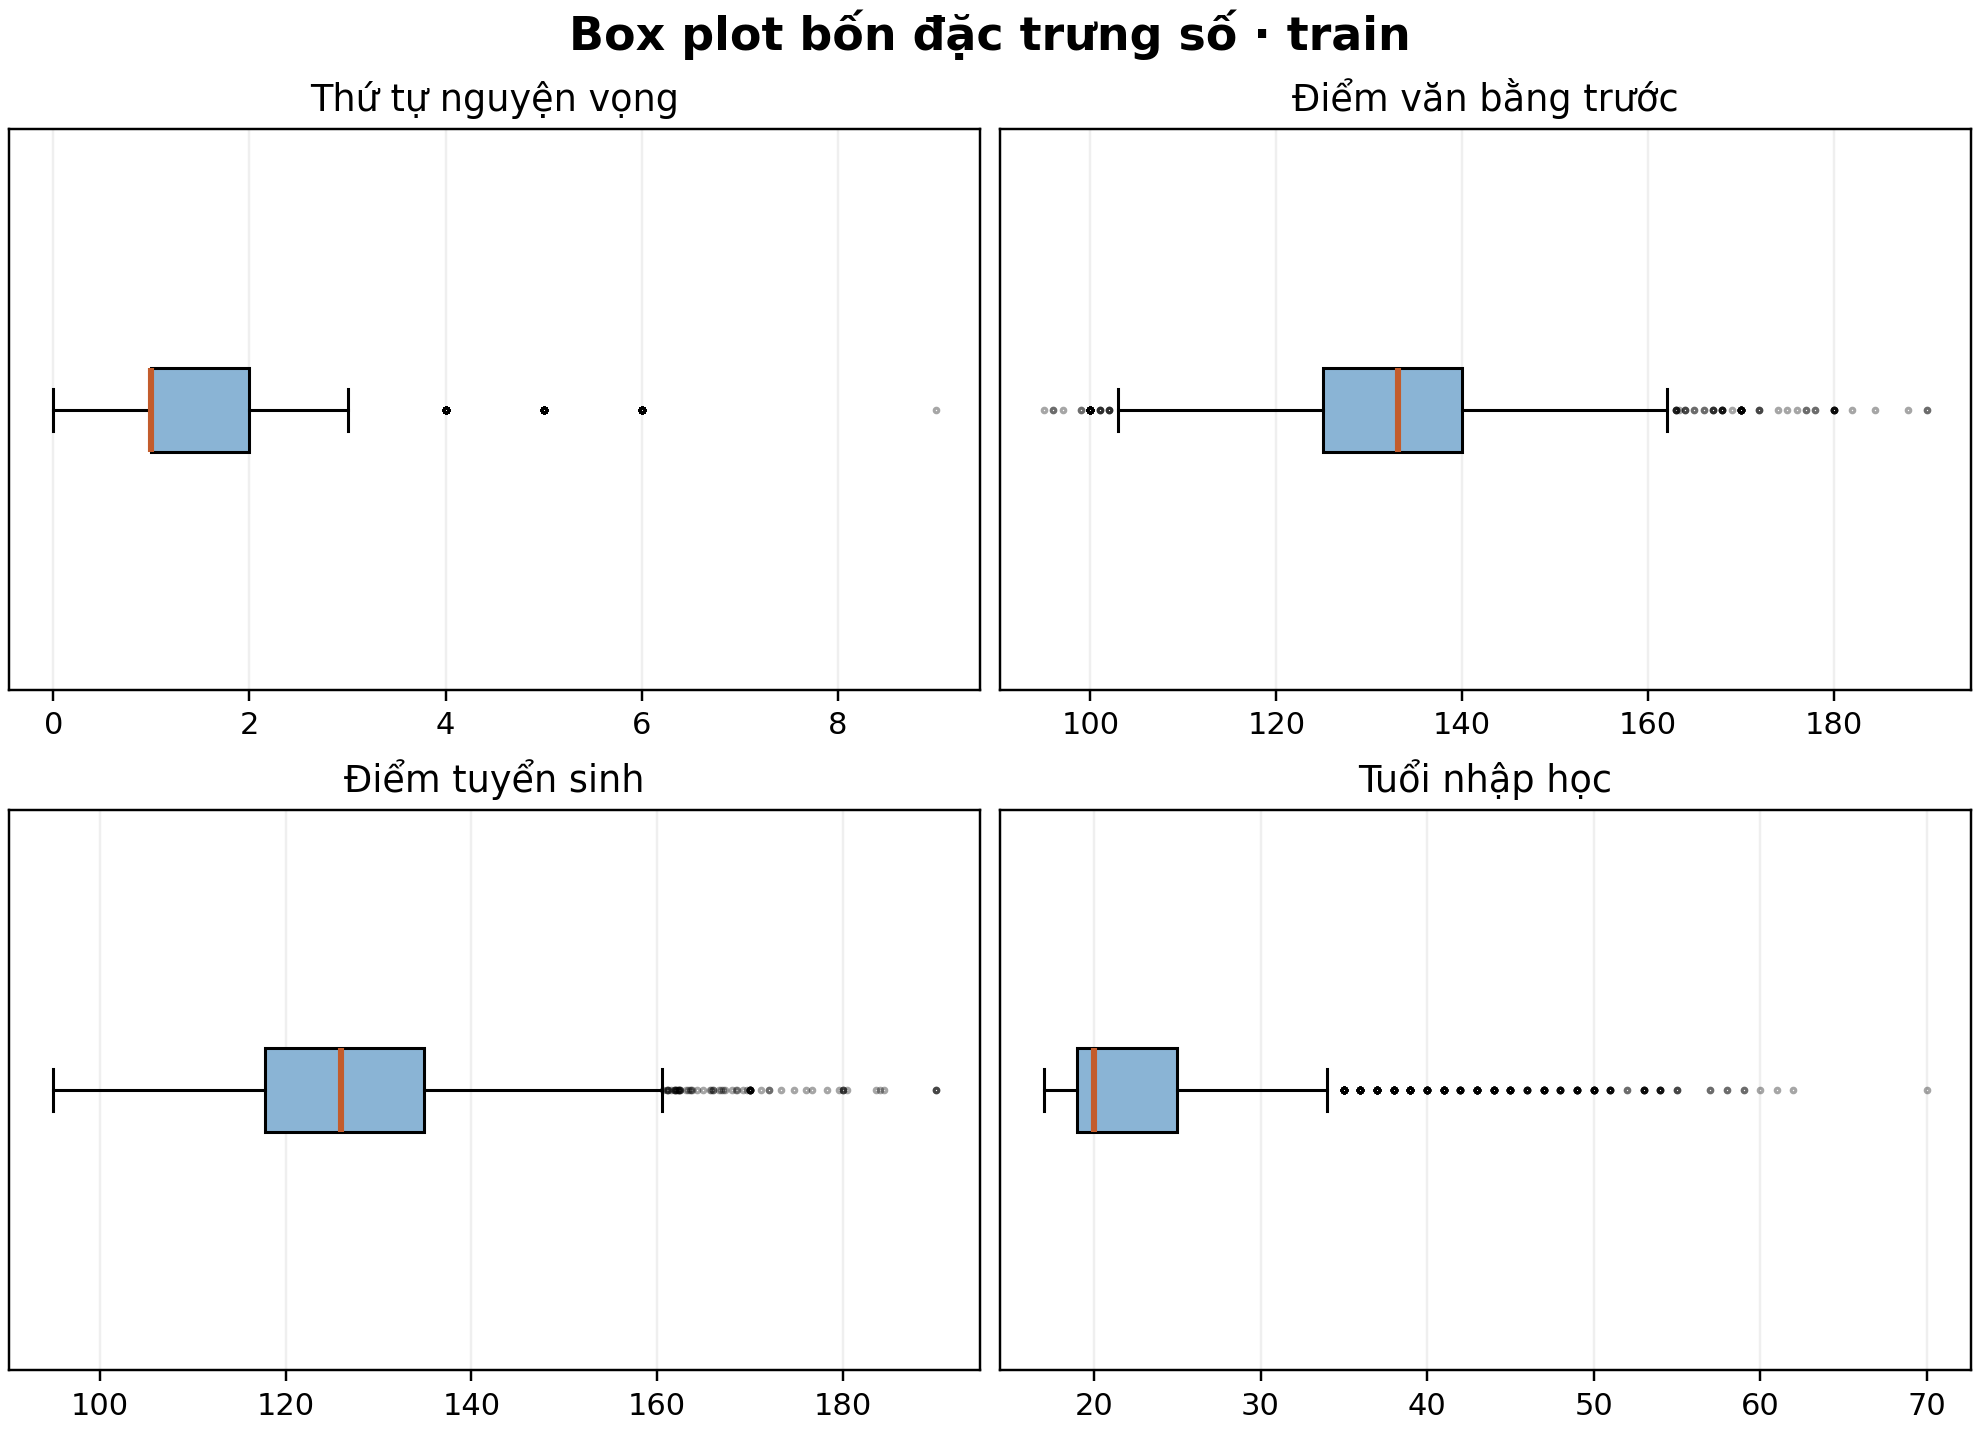
\includegraphics[width=\textwidth]{images/results/boxplots_numeric.png}
\caption{Box plot các biến số trên tập train; vạch màu là trung vị, hộp là khoảng IQR; râu tới điểm quan sát xa nhất trong ngưỡng $1{,}5\times\text{IQR}$, chấm là ngoại lệ.}\label{fig:boxplots}
\end{figure}

\subsection{Tương quan giữa các biến số}
Điểm văn bằng trước và điểm tuyển sinh có hệ số tương quan Pearson khoảng 0,581 trên train. Hai biến có liên hệ cùng chiều ở mức vừa trong tập này, nhưng tương quan không chứng minh biến này gây ra biến kia. Tuổi và thứ tự nguyện vọng có tương quan khoảng $-0{,}270$. Nhóm giữ cả bốn biến số vì những thống kê này chưa đủ căn cứ để loại bỏ biến nào.
\begin{figure}[H]\centering
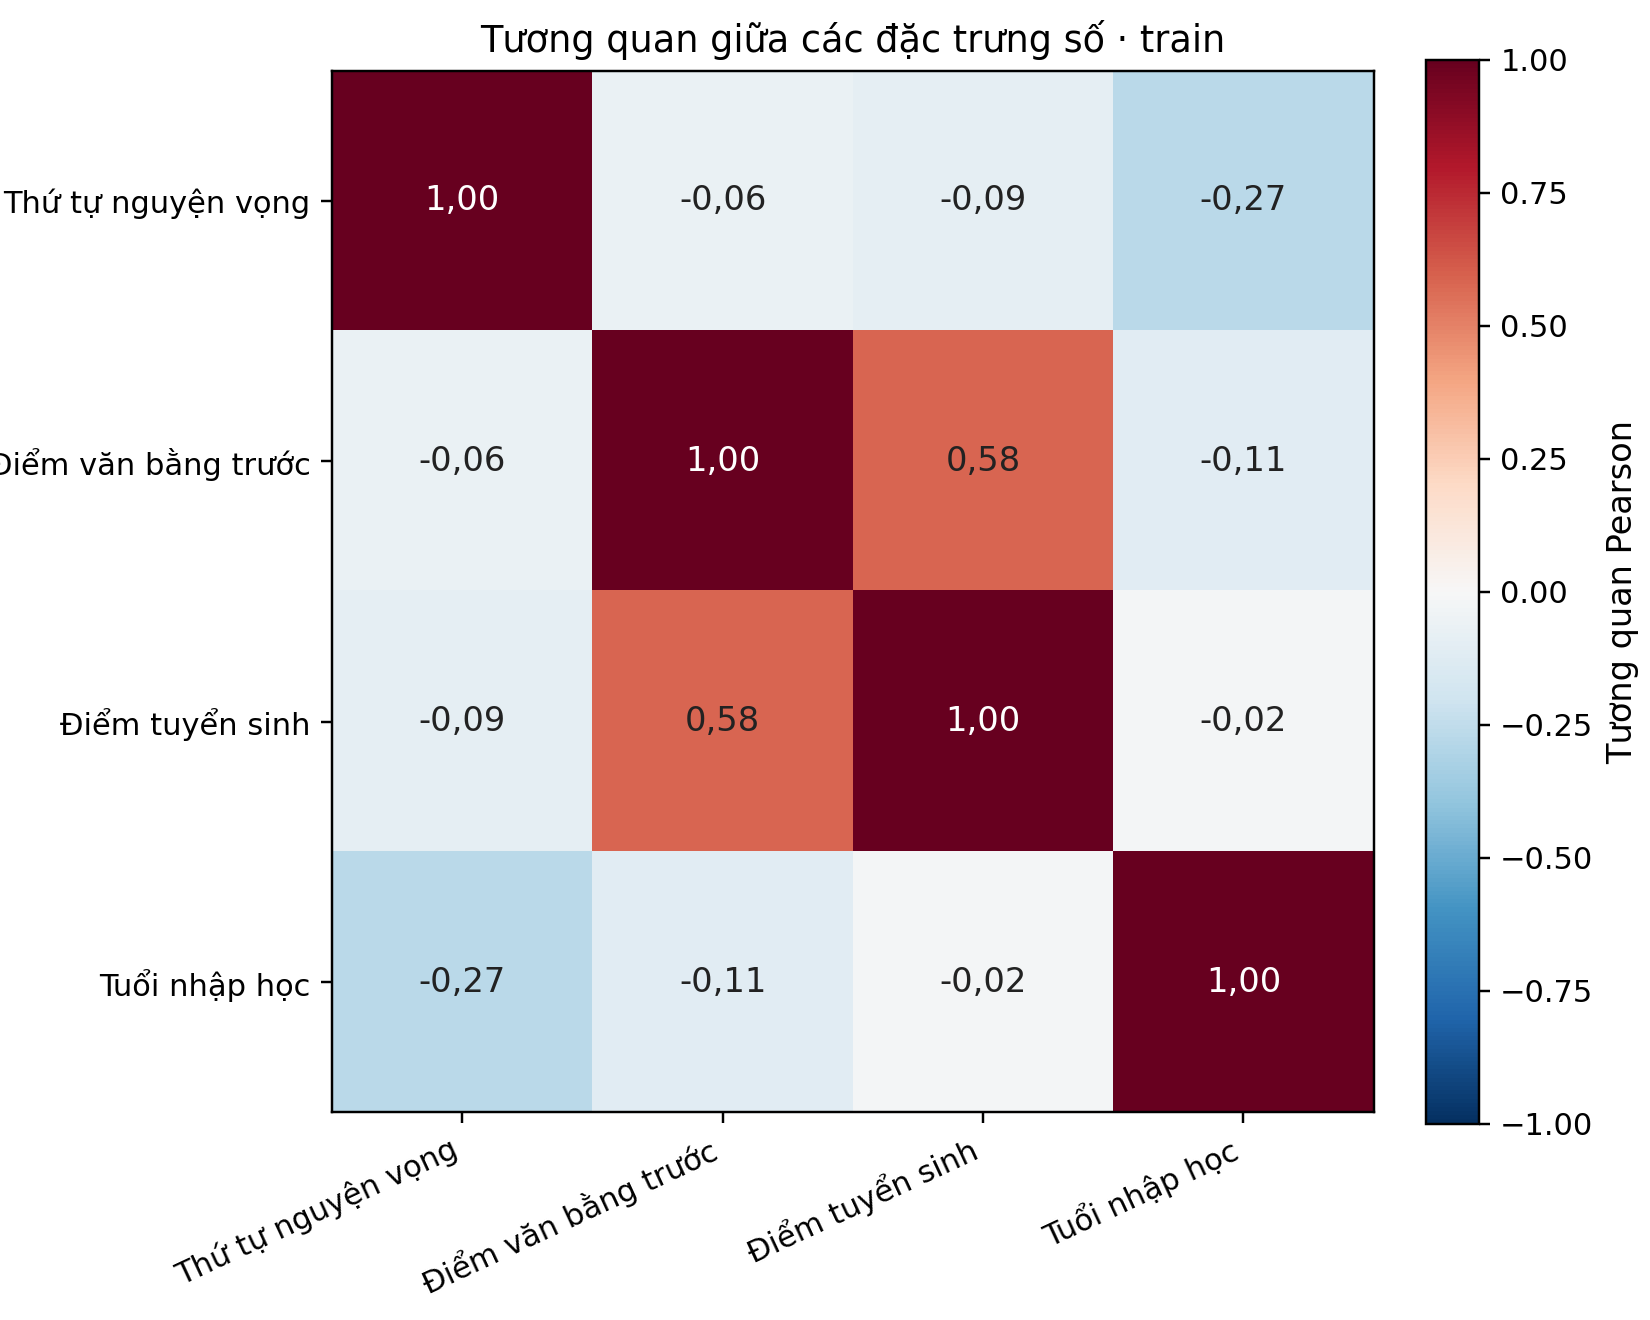
\includegraphics[width=.65\textwidth]{images/results/correlation_heatmap.png}
\caption{Heatmap tương quan Pearson giữa 4 biến số (tập train). Giá trị trong ô là hệ số tương quan.}\label{fig:corr}
\end{figure}
\begin{table}[H]\centering\small
\caption{Ma trận tương quan Pearson giữa 4 biến số (tập train)}\label{tab:corr}
\begin{tabular}{lrrrr}\toprule
 & App.Order & Prev.Grade & Adm.Grade & Age\\\midrule
Application order & 1,000 & $-$0,064 & $-$0,092 & $-$0,270\\
Previous grade & $-$0,064 & 1,000 & 0,581 & $-$0,112\\
Admission grade & $-$0,092 & 0,581 & 1,000 & $-$0,019\\
Age at enrollment & $-$0,270 & $-$0,112 & $-$0,019 & 1,000\\\bottomrule
\end{tabular}
\end{table}

\subsection{Biến phân loại}
Các cột phân loại cần được hiểu theo ý nghĩa, không theo kiểu lưu trữ. Ví dụ, \texttt{Course} được lưu dưới dạng số nhưng đó là mã ngành, không phải một đại lượng có thể so sánh hơn kém. Trong tập train, mã ngành 9500 có 607 mẫu; các ngành còn lại có số lượng khác nhau như Hình \ref{fig:courses}. Mã hiếm cung cấp ít ví dụ hơn cho mô hình học, nhất là khi chia thành nhiều fold.
\begin{figure}[H]\centering
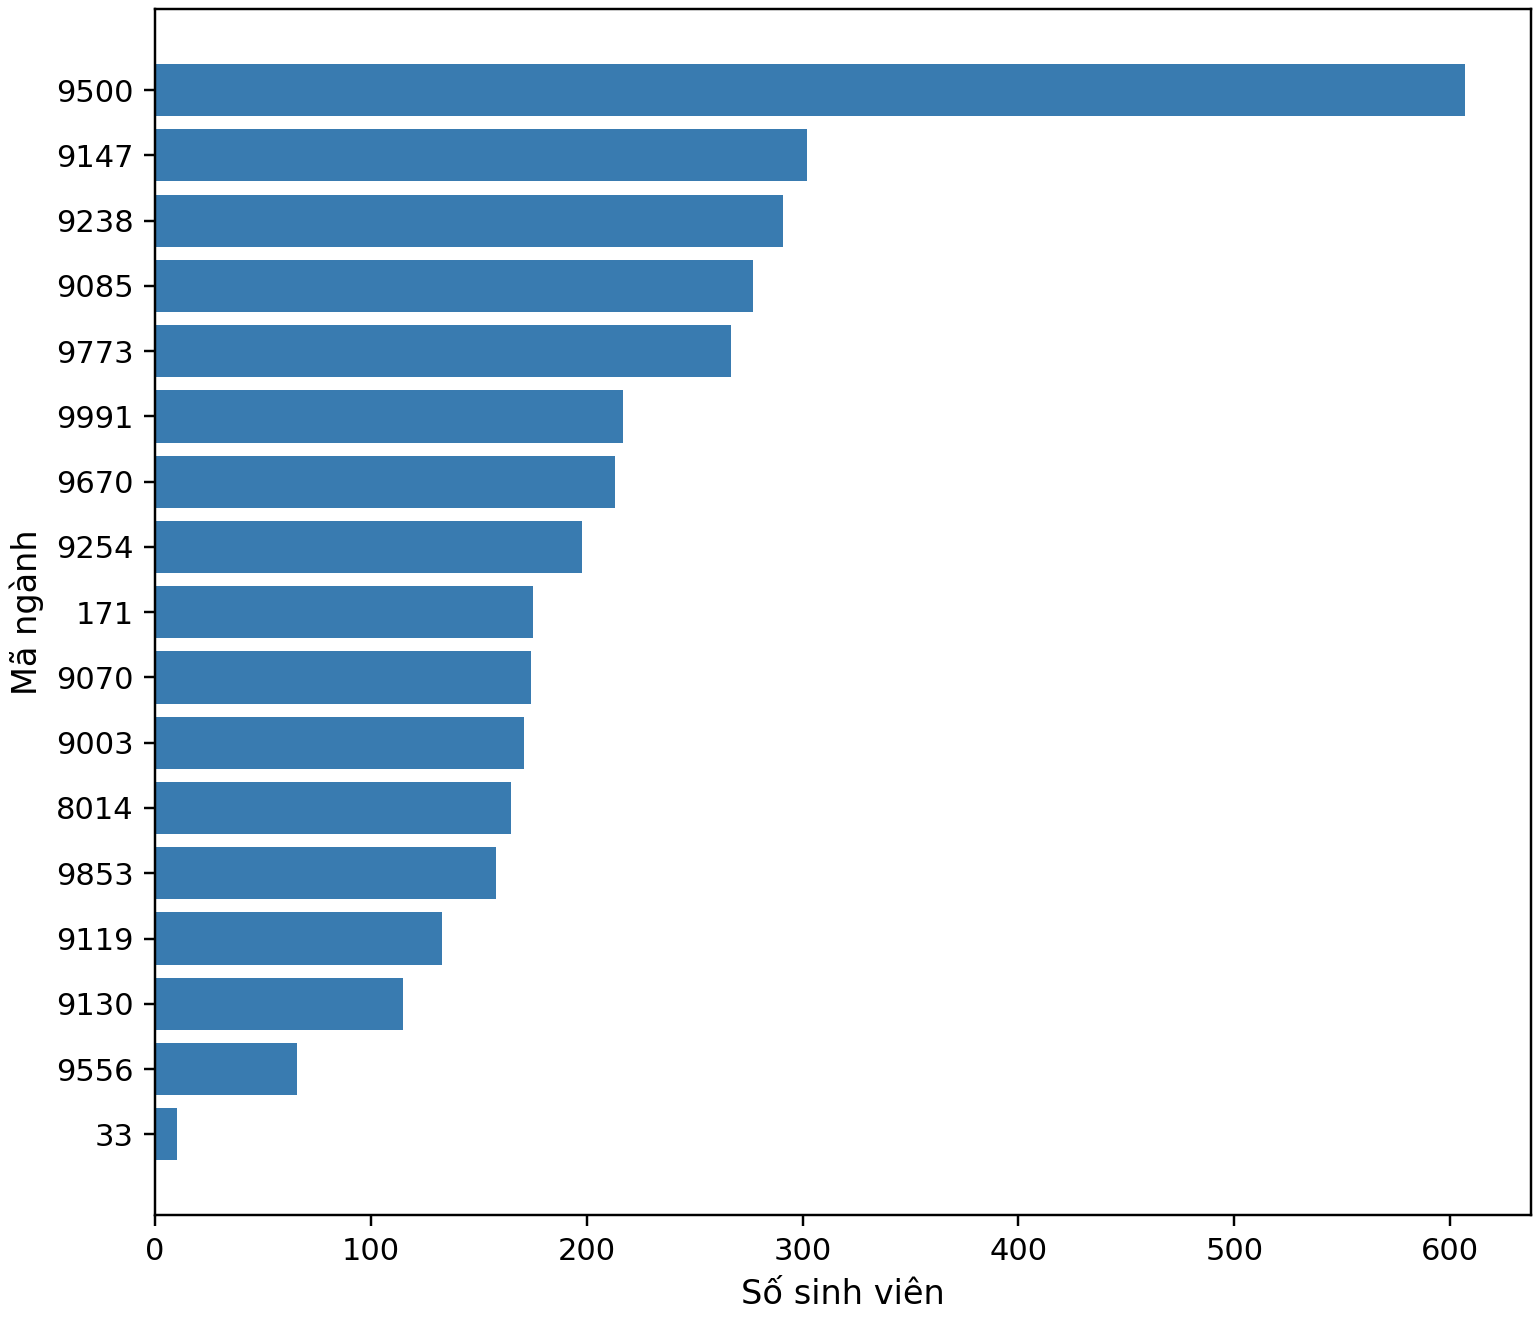
\includegraphics[width=.80\textwidth]{images/results/courses.png}
\caption{Số mẫu theo mã ngành trong tập train}\label{fig:courses}
\end{figure}
\begin{figure}[H]\centering
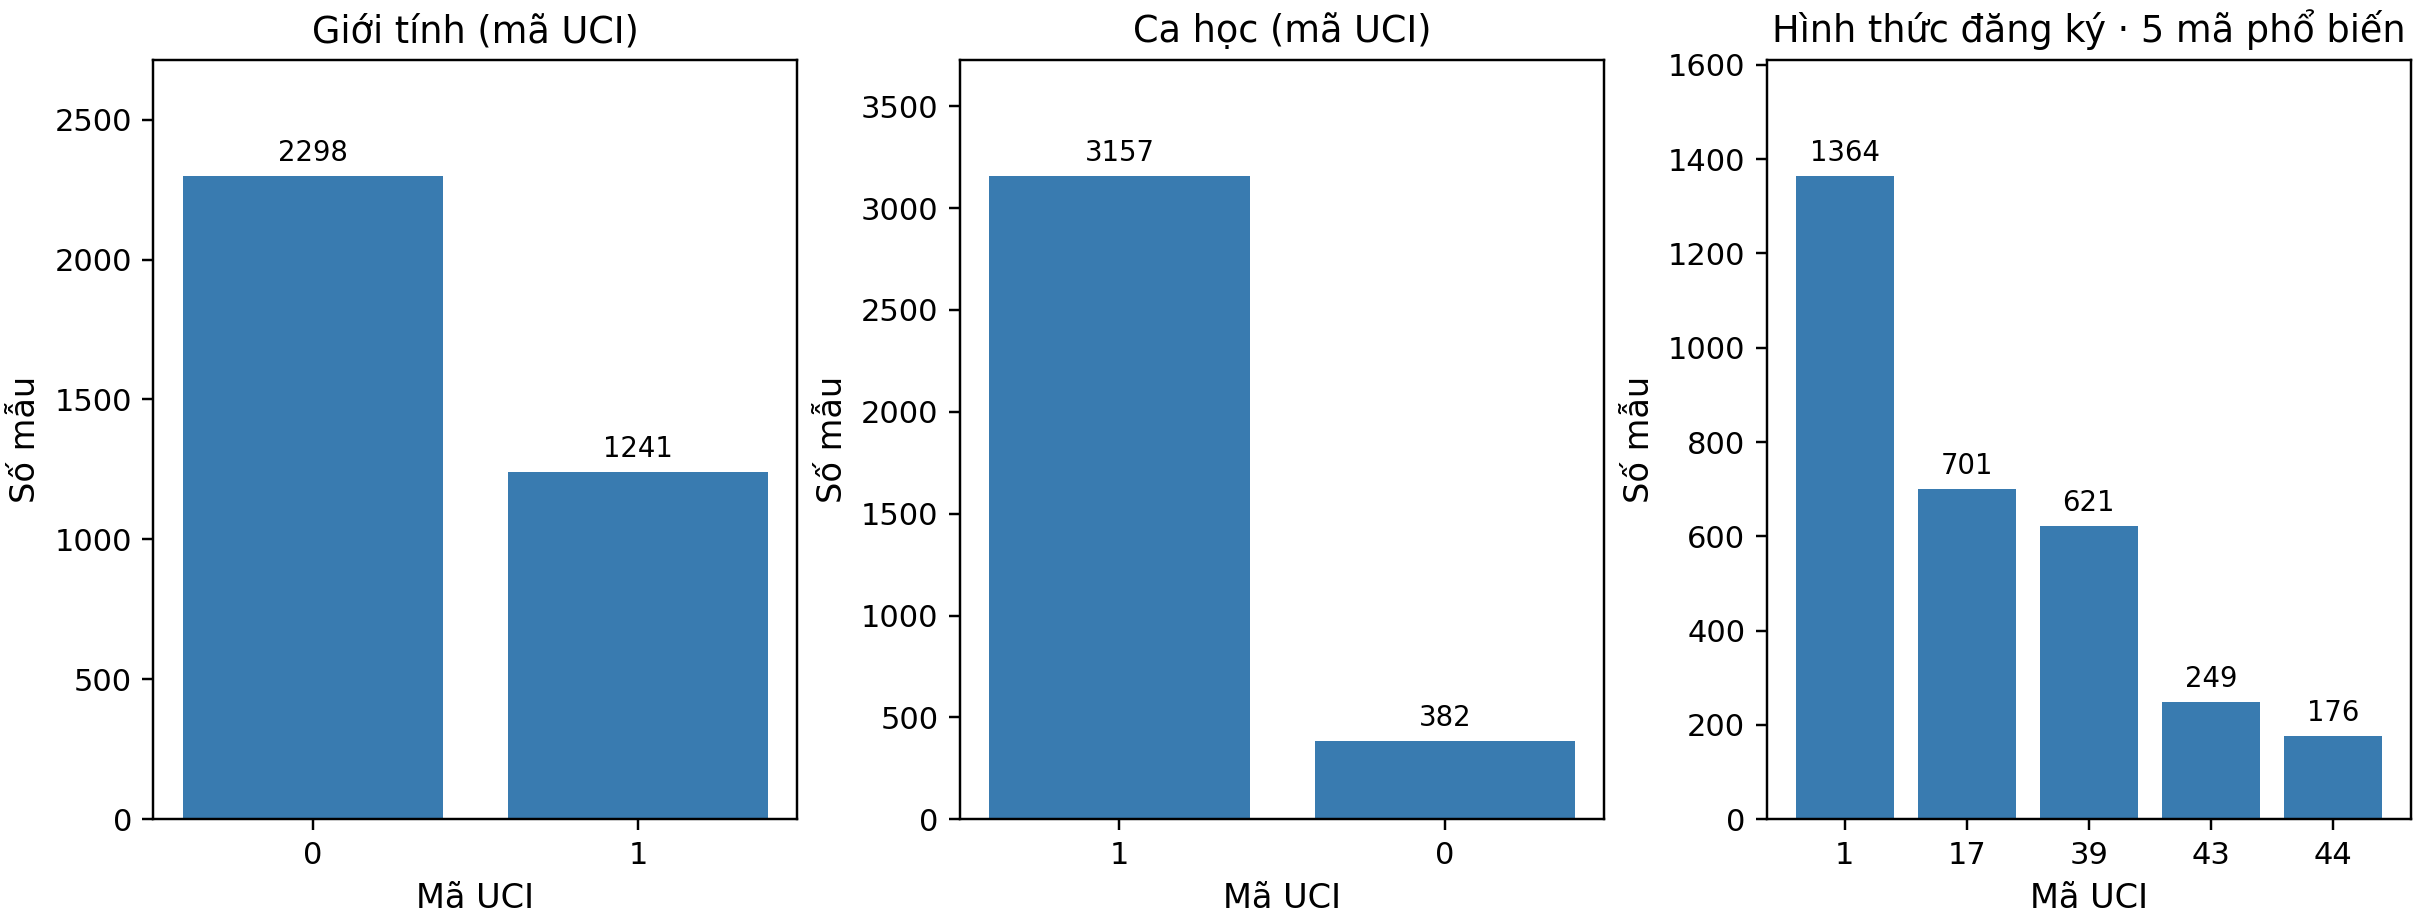
\includegraphics[width=\textwidth]{images/results/categorical_distributions.png}
\caption{Phân bố các biến phân loại chính (tập train): giới tính, ca học và hình thức đăng ký (top~5 mã). Nhãn cột ghi số lượng mẫu tương ứng.}\label{fig:cat-dist}
\end{figure}

\section{Thông tin thiếu và giới hạn của dữ liệu}
Không có ô trống không đồng nghĩa với việc mọi thông tin đều đầy đủ. Trong bảng mã UCI, giá trị 34 ở trình độ của cha hoặc mẹ có nghĩa là không rõ; tệp có 130 trường hợp ở cột của mẹ và 112 ở cột của cha. Giá trị 99 ở nghề nghiệp được mô tả là trống; số lần xuất hiện tương ứng là 17 và 19. Các con số này đếm từng cột nên không được cộng trực tiếp để suy ra số sinh viên khác nhau.

Trong chương trình, các mã trên được giữ như một nhóm phân loại riêng, không bị thay bằng giá trị phổ biến nhất. Cách này tránh tự đoán thông tin chưa biết, nhưng cũng có thể khiến mô hình học cả đặc điểm của quá trình thu thập dữ liệu. Nhóm ghi nhận đây là hạn chế, không khẳng định cách xử lý này tốt nhất khi chưa có thí nghiệm bổ sung.

Tập dữ liệu được lấy từ một cơ sở giáo dục, vì vậy kết quả không thể tự động đại diện cho các trường khác. Trong tập train còn có những nhóm nhỏ: 86 sinh viên có mã quốc tế và 41 sinh viên có mã nhu cầu giáo dục đặc biệt. Những nhóm ít mẫu cần được nghiên cứu cẩn thận hơn nếu muốn đánh giá mô hình theo từng nhóm; bài tập hiện chưa thực hiện đánh giá công bằng đó.

\section{Phân tích cột gây rò rỉ nhãn}\label{sec:leakage}
Một rủi ro quan trọng khi đặt bài toán dự đoán tại thời điểm nhập học là rò rỉ thông tin tương lai (data leakage): đưa vào mô hình những cột chỉ có thể biết \emph{sau} khi sinh viên đã bắt đầu hoặc kết thúc quá trình học. Nhóm loại bỏ 12 cột học kỳ chưa có lúc nhập học và 6 cột có thời điểm ghi nhận chưa được xác nhận:

\begin{itemize}
  \item \textbf{Kết quả học kỳ 1 và 2} (12 cột: số tín chỉ đã công nhận, đã đăng ký, đã đánh giá, đã hoàn thành, điểm trung bình và số tín chỉ không đánh giá của từng học kỳ): các thông tin này chỉ phát sinh sau khi sinh viên đã theo học ít nhất một hoặc hai kỳ; đưa vào sẽ biến bài toán thành dự đoán \emph{sau sự kiện}.
  \item \textbf{Debtor} (nợ học phí): phát sinh trong quá trình học tập; không xác định được thời điểm ghi nhận trong hồ sơ nhập học.
  \item \textbf{Tuition fees up to date} (tình trạng cập nhật học phí): phụ thuộc vào quá trình đóng học phí định kỳ sau khi đã nhập học.
  \item \textbf{Scholarship holder} (học bổng): nhiều trường hợp học bổng được xét duyệt sau khi đã có kết quả xét tuyển hoặc trong quá trình học.
  \item \textbf{Unemployment rate, Inflation rate, GDP}: thời điểm ghi nhận hoặc công bố của các chỉ số này chưa được xác nhận so với thời điểm dự đoán; chúng bị loại theo nguyên tắc thận trọng.
\end{itemize}

Để minh chứng tác động thực tế của rò rỉ thông tin, nhóm thực hiện thí nghiệm so sánh trực tiếp trên cùng tập train với 5-fold CV phân tầng (giữ nguyên mô hình Cây quyết định mặc định không giới hạn độ sâu):
\begin{itemize}
  \item \textbf{Khi sử dụng toàn bộ 36 đặc trưng} (bao gồm các cột học kỳ và tài chính): Macro-F1 CV đạt $0{,}6265 \pm 0{,}0143$ (accuracy CV $0{,}6869$).
  \item \textbf{Khi chỉ sử dụng 18 đặc trưng nhập học} (không dùng 18 cột được liệt kê): Macro-F1 CV giảm xuống $0{,}4241 \pm 0{,}0205$.
\end{itemize}
Chênh lệch 0,2024 điểm macro-F1 cho thấy toàn bộ 18 cột bổ sung chứa thông tin dự báo. Thí nghiệm thêm cả 18 cột cùng lúc nên không quy riêng mức tăng cho học kỳ hay học phí. Đối với dự đoán lúc nhập học, cột học kỳ là thông tin tương lai; thời điểm của các cột còn lại cần xác minh. Độ lệch sau dấu $\pm$ là độ lệch chuẩn giữa năm fold, không phải khoảng tin cậy. Kịch bản 36 cột chỉ để minh họa và không dùng lựa chọn mô hình.

\section{Quan hệ đặc trưng và nhãn trên train và giả thuyết ban đầu}
Hình~\ref{fig:dropout-group} thể hiện tỷ lệ Dropout trong các nhóm ngành, độ tuổi và hình thức đăng ký trên tập train (kèm số lượng mẫu tương ứng).
\begin{figure}[H]\centering
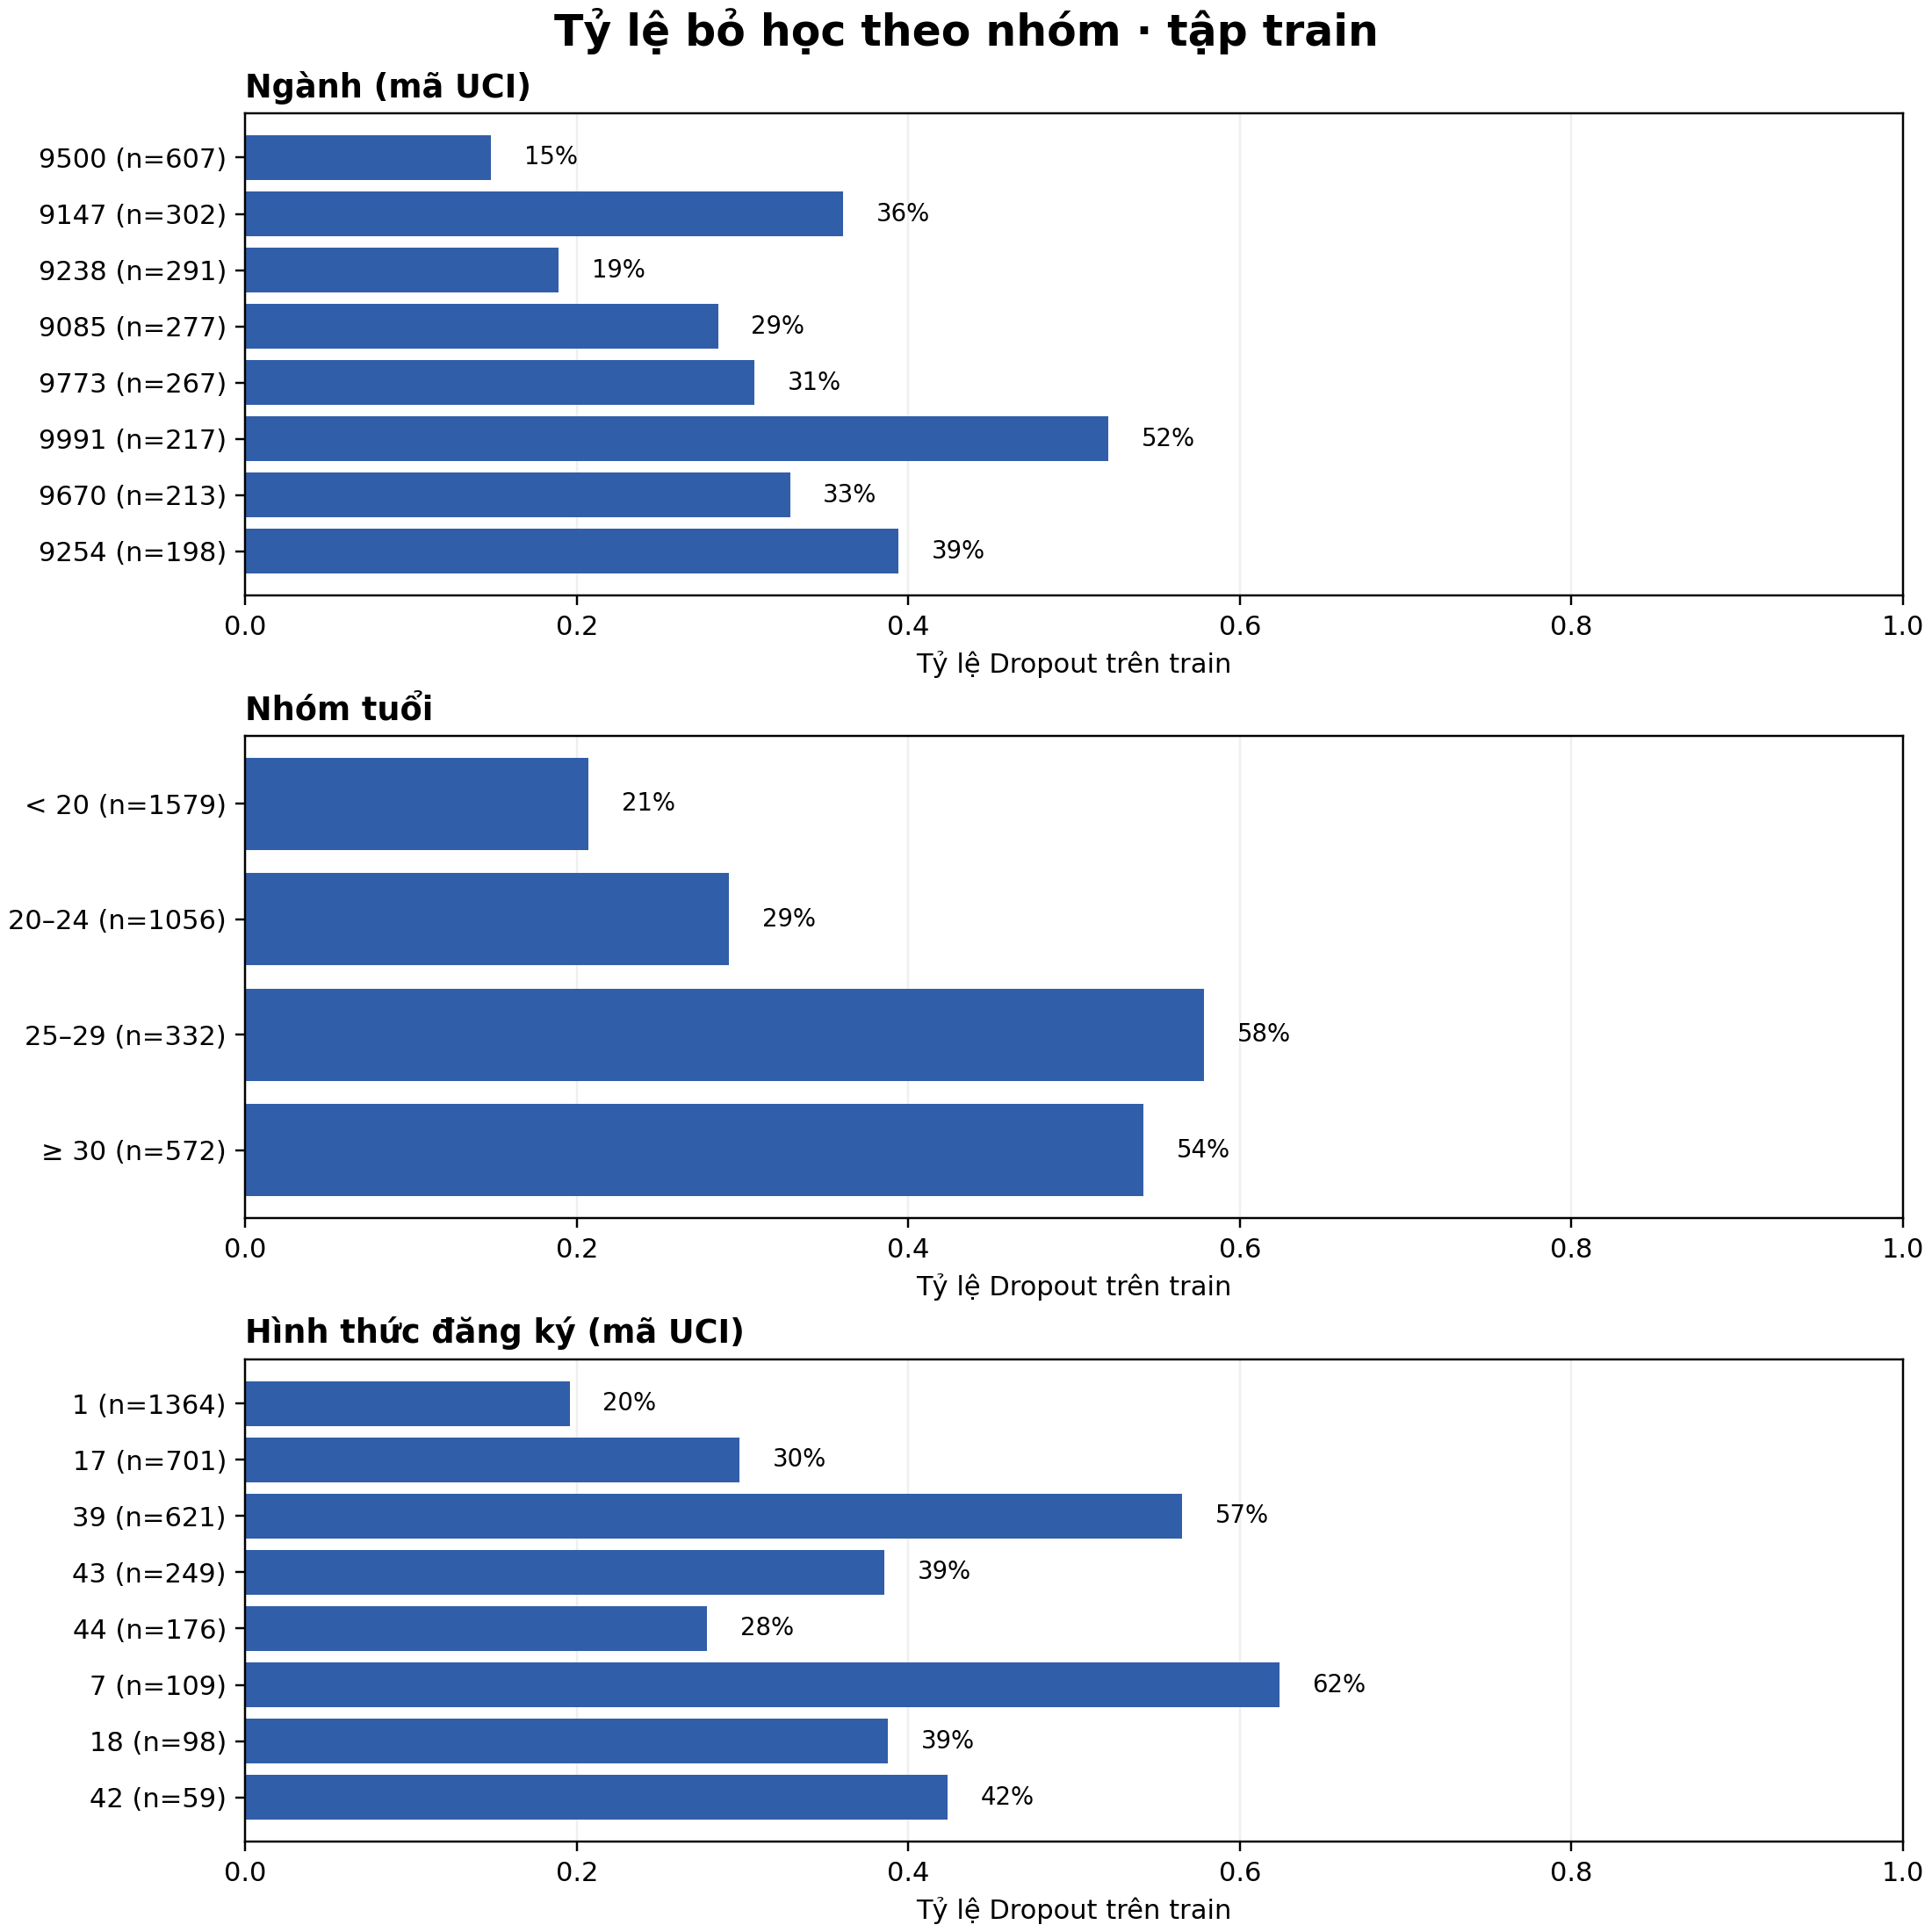
\includegraphics[width=\textwidth]{images/results/dropout_by_group.png}
\caption{Tỷ lệ Dropout theo nhóm trên tập train (ngành và hình thức đăng ký hiển thị các mã phổ biến nhất).}\label{fig:dropout-group}
\end{figure}

Từ phân tích trực quan này, nhóm hình thành các giả thuyết ban đầu cho việc kỹ thuật đặc trưng và mô hình hóa:
\begin{enumerate}
  \item \textbf{Giả thuyết về độ tuổi nhập học}: Sinh viên dưới 20 tuổi có tỷ lệ Dropout thấp nhất (20,7\% với 327/1.579 mẫu), trong khi nhóm 20--24 tuổi là 29,2\% và nhóm 25--29 tuổi lên tới 57,8\% (192/332 mẫu). Áp lực việc làm hoặc gia đình là giả thuyết cần kiểm tra thêm; dữ liệu hiện tại không xác nhận nguyên nhân này. Do đó, việc chia nhóm tuổi (\texttt{age\_band}) có thể cung cấp ngưỡng phân tách phi tuyến tốt hơn cho mô hình.
  \item \textbf{Giả thuyết về ngành học}: Tỷ lệ bỏ học có sự phân hóa mạnh giữa các ngành: ví dụ mã ngành 9500 (Điều dưỡng) có tỷ lệ bỏ học thấp (khoảng 14,8\%), trong khi mã ngành 9147 (Quản lý) có tỷ lệ bỏ học khoảng 36,1\%. Sự khác biệt gợi ý khảo sát thêm vai trò ngành; không chứng minh ngành gây ra bỏ học.
  \item \textbf{Giả thuyết về chênh lệch điểm số}: Mối tương quan 0,581 giữa điểm tuyển sinh và điểm văn bằng trước cho thấy xu hướng chung, nhưng các trường hợp chênh lệch âm lớn (điểm tuyển sinh thấp hơn đáng kể so với điểm học bạ trước đó) có thể phản ánh khác biệt giữa hai lần đánh giá; nguyên nhân chưa được xác minh. Biến hiệu số (\texttt{Admission grade - Previous grade}) được đề xuất để nắm bắt yếu tố này.
\end{enumerate}
